\selectlanguage{italian}

\section{Principio variazionale di Ritz}

Per lo studio di un sistema quantistico, è utile dimostrare un principio variazionale sul valore di aspettazione dell'Hamiltoniana $ \mathcal{H} $ del sistema, ovvero sull'energia:
\begin{equation}
	E[\psi] \defeq \frac{\braket{\psi | \mathcal{H} | \psi}}{\braket{\psi | \psi}} \in \R
\end{equation}

\begin{proposition}{}{}
	Il valore di aspettazione di una Hamiltoniana su un suo autostato è stazionario.

	\tcblower

	\begin{proof}
		Prendendo una variazione infinitesima $ \ket{\psi + \delta\psi} $ ed usando $ \mathcal{H} \ket{\psi} = E[\psi] \ket{\psi} $:
		\begin{equation*}
			\begin{split}
				\delta E
				&= E[\psi + \delta\psi] - E[\psi] = \frac{\braket{\psi + \delta\psi | \mathcal{H} | \psi + \delta\psi}}{\braket{\psi + \delta\psi | \psi + \delta\psi}} - \frac{\braket{\psi | \mathcal{H} | \psi}}{\braket{\psi | \psi}} \\
				&\simeq \frac{\braket{\psi | \mathcal{H} | \psi} + \braket{\psi | \mathcal{H} | \delta\psi} + \braket{\delta\psi | \mathcal{H} | \psi}}{\braket{\psi | \psi} + \braket{\psi | \delta\psi} + \braket{\delta\psi | \psi}} - \frac{\braket{\psi | \mathcal{H} | \psi}}{\braket{\psi | \psi}} \\
				&= \frac{\braket{\psi | \mathcal{H} | \delta\psi} + \braket{\delta\psi | \mathcal{H} | \psi} - E[\psi] \braket{\psi | \delta\psi} - E[\psi] \braket{\delta\psi | \psi}}{\braket{\psi | \psi} + \braket{\psi | \delta\psi} + \braket{\delta\psi | \psi}} \\
				&= \frac{2\Re \braket{\delta\psi | (\mathcal{H} - E[\psi]) | \psi}}{\braket{\psi | \psi} + \braket{\psi | \delta\psi} + \braket{\delta\psi | \psi}} = 0
			\end{split}
		\end{equation*}
	\end{proof}
\end{proposition}

\begin{theorem}{Principio variazionale di Ritz}{ritz}
	Detto $ \ket{\psi_0} $ lo stato fondamentale di $ \mathcal{H} $, allora $ E[\psi] \ge E[\psi_0] \equiv E_0 \,\,\forall \ket{\psi} \in \mathscr{H} $.

	\tcblower
	\begin{proof}
		Data una base di autostati $ \{u_n\} : \mathcal{H} \ket{u_n} = E_n \ket{u_n} \land \braket{u_n | u_m} = \delta_{nm} $, dove $ u_0 $ è il ground state con $ E_0 \le E_1 \le E_2 \le \dots $, per il generico stato $ \ket{\psi} = \sum_n A_n \ket{u_n} $:
		\begin{equation*}
			E[\psi] - E_0
			= \frac{\abs{A_0}^2 E_0 + \sum_{i \neq 0} \abs{A_i}^2 E_i}{\abs{A_0}^2 + \sum_{i \neq 0} \abs{A_i}^2} - E_0 = \frac{\sum_{i \neq 0} \left( E_i - E_0 \right) \abs{A_i}^2}{\abs{A_0}^2 + \sum_{i \neq 0} \abs{A_i}^2} \ge 0
		\end{equation*}
	\end{proof}
\end{theorem}

Questo risultato è utile poiché permette di trovare il ground state minimizzando l'energia: se si parametrizza la funzione d'onda, il ground state sarà dato dal set di parametri per cui si ha il minimo dell'energia.\\
Una possibile applicazione è quella di ottimizzare i coefficienti di uno sviluppo di una funzione d'onda su una base di funzioni d'onda fissate: vedendo i coefficienti della combinazione lineare come parametri, minimizzando l'energia si ottiene un sistema lineare di equazioni la cui risoluzione fornisce i parametri che meglio approssimano la funzione d'onda reale. Questo è il caso, ad esempio, della Linear Combination of Atomic Orbital, nel quale si esprime la funzione d'onda di una molecola come combinazione lineare delle funzioni d'onda dei suoi atomi costituenti.\\
Questo metodo può essere ulteriormente generalizzato facendo variare parametricamente anche le funzioni d'onda di base sulle quali si effettua lo sviluppo (es.: metodo di Hartree-Fock).

\section{Soluzione analitica}

L'atomo a singolo elettrone (o idrogenoide) è uno dei pochi casi in cui l'equazione di Schrödinger può essere risolta analiticamente. Essendo il potenziale coulombiano un potenziale radiale a simmetria sferica, si può separare il problema in moto del centro di massa e moto radiale: essendo la massa nucleo $ M $ migliaia di volte quella dell'elettrone $ m_e $, il centro di massa può essere approssimato con la posizione stessa del nucleo. La correzione di massa ridotta diventa importante quando si considerano atomi esotici, come ad esempio l'idrogeno muonico (sistema legato protone-muone).\\
Concentrandosi sull'Hamiltoniana di moto relativo (quella del centro di massa è semplicemente l'Hamiltoniana di particella libera):
\begin{equation}
	\mathcal{H} = - \frac{\hbar^2}{2\mu} \nabla_\ve{r}^2 - \frac{Ze}{r}
	\label{eq:1-e-ham}
\end{equation}
dove $ \ve{r} \equiv \ve{R} - \ve{r}_e $ e $ \mu \equiv (M^{-1} + m_e^{-1})^{-1} $. In coordinate sferiche si trova:
\begin{equation*}
	\nabla^2 = \frac{2}{r} \frac{\pa}{\pa r} + \frac{\pa^2}{\pa r^2} - \frac{\hat{L}^2}{\hbar^2 r^2}
\end{equation*}
Dato che $ [\mathcal{H} , \hat{L}^2] = 0 $, si può cercare una soluzione $ \psi = \psi(r,\vartheta,\varphi) $ in funzione delle autofunzioni di $ \hat{L}^2 $: questi sono le armoniche sferiche $ Y_{\ell,m} : \hat{L}^2 Y_{\ell,m} = \hbar^2 \ell (\ell + 1) Y_{\ell,m} $, con $ \ell \in \N_0 $ e $ -\ell \le m \le \ell $. Scrivendo $ \psi(r,\vartheta,\varphi) = R(r) Y_{\ell,m}(\vartheta,\varphi) $ si ha:
\begin{equation}
	\left[ - \frac{\hbar^2}{2\mu} \left( \frac{2}{r} \frac{\dd}{\dd r} + \frac{\dd^2}{\dd r^2} \right) + V_\ell(r) \right] R(r) = E R(r)
	\qquad \qquad
	V_\ell(r) \equiv - \frac{Ze}{r} + \frac{\hbar^2 \ell(\ell + 1)}{2\mu r^2}
	\label{eq:1-e-rad-eq}
\end{equation}
Risolvendo questa equazione si trova che la funzione d'onda radiale dipende da un numero quantico, il \textit{numero quantico radiale} $ n_r $, tale per cui:
\begin{equation*}
	E_{n_r,\ell} = - \frac{Z^2 e^4 \mu}{2\hbar^2 (n_r + \ell + 1)^2}
\end{equation*}
Questo numero quantico rappresenta il numero di nodi nella funzione d'onda radiale $ R_{n_r,\ell}(r) $, nel caso di un potenziale radiale a simmetria sferica. Conviene definire un numero quantico equivalente, il \textit{numero quantico principale} $ n \equiv n_r + \ell + 1 $, così che:
\begin{equation}
	E_n = - \frac{Z^2 e^4 \mu}{2\hbar^2} \frac{1}{n^2} = - \frac{Z^2}{2} E_\text{Ha} \frac{\mu}{m_e} \frac{1}{n^2}
	\label{eq:1-e-en}
\end{equation}
Vale inoltre che $ 0 \le \ell \le n-1 $.

\paragraph{Degenerazione}

Dallo spettro energetico Eq. \ref{eq:1-e-en} si vede che l'energia non dipende né da $ m $ né da $ \ell $: nel primo caso si parla di \textit{degenerazione necessaria}, in quanto è una degenerazione dovuta alla simmetria sferica del problema e comporta $ d(\ell) = 2\ell + 1 $, mentre nel secondo caso di ha una \textit{degenerazione accidentale}, legata alla forma particolare del potenziale coulombiano. La presenza di quest'ultima degenerazione accidentale permette di definire il numero quantico principale, e si ha una degenerazione overall di $ d(n) = \sum_{\ell = 0}^{n-1} (2\ell + 1) = n^2 $.

\subsection{Funzione d'onda angolare}

L'armonica sferica $ Y_{\ell,m}(\vartheta,\varphi) $ contiene informazione esatta sul momento angolare totale e sulla sua proiezione sull'asse $ z $, in quanto $ \hat{L}^2 Y_{\ell,m} = \hbar^2 \ell (\ell + 1) $ e $ \hat{L}_z Y_{\ell,m} = \hbar m $, mentre quella sul momento angolare lungo le altre direzioni è di natura probabilistica, poiché $ [\hat{L}_x , \hat{L}_z],[\hat{L}_y , \hat{L}_z] \neq 0 $. Si noti, però, che grazie alla simmetria sferica la definizione di $ \ve{e}_z $ è arbitraria.\\
La forma generica di un'armonica sferica è data da:
\begin{equation}
	Y_{\ell,m}(\vartheta,\varphi) = \mathcal{N} e^{i m \varphi} P_\ell^{\abs{m}}(\cos \vartheta)
\end{equation}
dove $ P_\ell^{\abs{m}}(\cos \vartheta) $ è la funzione di Legendre. Si vede dunque che $ \abs{Y_{\ell,m}}^2 $ è indipendente da $ \varphi $, dunque la probabilità $ \abs{\braket{\vartheta,\varphi | n,\ell,m}}^2 $ dipende solo da $ \vartheta $. Inoltre, si trova che $ \ell - \abs{m} $ è pari al numero di nodi della funzione di Legendre, e che sotto operatore di parità $ \mathcal{P} Y_{\ell,m} = (-1)^\ell Y_{\ell,m} $.\\
Data la simmetria necessaria rispetto ad $ m $, si possono combinare orbitali con $ \pm m $ per ottenere degli orbitali reali: $ Y_{0,0} = \frac{1}{\sqrt{4\pi}} $ e $ Y_{\ell,0} \propto \cos{\vartheta} $ sono sempre reali, mentre ad esempio si definiscono gli orbitali reali $ \ch{p}_x , \ch{p}_y $ come:
\begin{equation*}
	\psi_{\ch{p}_x} = \frac{1}{\sqrt{2}} \left( Y_{1,-1} - Y_{1,1} \right)
	\qquad \qquad
	\psi_{\ch{p}_y} = \frac{i}{2} \left( Y_{1,-1} + Y_{1,1} \right)
\end{equation*}

\subsection{Funzione d'onda radiale}

Per quanto riguarda la funzione d'onda radiale $ R_{n_r,\ell}(r) $, essa ha la forma generica:
\begin{equation}
	R_{n,\ell}(r) = \mathcal{N} (kr)^\ell L_{n+\ell}^{2\ell + 1}(kr) e^{-\frac{1}{2} kr}
	\qquad
	k \equiv \frac{2Z}{a} \frac{1}{n}
	\label{eq:1-e-radial}
\end{equation}
dove $ L_{n+\ell}^{2\ell+1}(kr) $ è il polinomio di Laguerre, un polinomio di grado $ n - \ell - 1 $ (con termine noto non-nullo) che presenta un numero di nodi pari a $ n - \ell - 1 $, ed $ a \equiv \frac{m_e}{\mu} a_0 $ è la mass-rescaled atomic length. Si vedono subito i due limiti:
\begin{equation*}
	\lim_{r \rightarrow 0} R_{n,\ell}(r) \sim r^\ell
	\qquad \qquad
	\lim_{r \rightarrow \infty} R_{n,\ell}(r) \sim r^{n-1} e^{-\frac{1}{2} kr}
\end{equation*}
La distribuzione di probabilità spaziale è data dunque da:
\begin{equation}
	P_{n,\ell,m}(\ve{r}) \dd^3r = \abs{R_{n,\ell}(r)}^2 \abs{Y_{\ell,m}(\vartheta,\varphi)}^2 r^2 \sin{\vartheta} \dd r \dd \vartheta \dd \varphi
\end{equation}
La probabilità $ P_{n,0,0}(\ve{r}) $ ha un massimo assoluto in $ \ve{r} = \ve{0} $: la posizione più probabile per l'elettrone nello stato $ \ch{s} $ è il centro del potenziale, dove esso è più attrattivo. Per $ \ell \neq 0 $, invece, $ P_{n,\ell,m}(\ve{0}) = 0 $, e ciò evidenzia l'impossibilità per una particella dotata di momento angolare di cadere nel centro di un potenziale centrale.\\
Si osserva inoltre che, all'aumentare di $ Z $, il massimo di $ \abs{R_{n,\ell}(r)}^2 $ e dunque di $ P_{n,\ell,m}(\ve{r}) $ si sposta verso l'origine\footnote{In particolare $ R_{n,\ell}^{[Z]}(r) = Z^{3/2} R_{n,\ell}^{[1]}(rZ) $, quindi $ P_{n,\ell,m}^{[Z]}(r) = Z P^{[1]}(rZ) $.}: ciò implica che la distanza elettrone-nucleo è $ \propto Z^{-1} $, dunque, dato che $ V \propto Z/r $, si trova l'andamento dell'energia $ E \propto Z^2 $.\\
La funzione d'onda più semplice, quello dello stato $ 1\ch{s} $, si trova essere:
\begin{equation}
	\psi_{1,0,0}(\ve{r}) = \frac{1}{\sqrt{\pi}} \left( \frac{Z}{a} \right)^{3/2} e^{- Z r / a}
\end{equation}

\section{Spettro energetico}

Quando si parla di spettro d'eccitazione si intende lo spettro delle differenze di autovalori di energia: dati due stati $ \ket{i} , \ket{f} $, si ha $ \Delta E = E_f - E_i $. Dall'Eq. \ref{eq:1-e-en} si trova:
\begin{equation}
	\Delta E = - \frac{\mu}{m_e} \frac{E_\text{Ha}}{2} Z^2 \left( \frac{1}{n_f^2} - \frac{1}{n_i^2} \right)
	\label{eq:1-e-spectr}
\end{equation}
Queste sono quantità misurabili spettroscopicamente.

\subsection{Atomo di idrogeno}

Per l'atomo di idrogeno si ha il ground state $ E_1 = - \frac{1}{2} E_\text{Ha} \frac{\mu}{m_e} = - 13.5983\ev $. Le transizioni $ n_i \rightarrow n_f $ si raggruppano in serie, ciascuna caratterizzata dallo stesso stato finale $ n_f $ ad energia più bassa: per l'atomo di idrogeno, ciascuna serie è osservata in una presisa regione caratteristica dello spettro elettromagnetico, ed in particolare le serie di Lyman ($ n_f = 1 $) e Balmer ($ n_f = 2 $) non presentano alcun overlap con altre serie, dato che la distanza energetica tra $ E_1 \simeq - 13.60\ev $ o $ E_2 \simeq -3.39\ev $ ed il successivo stato eccitato supera l'intero range energetico tra quest'ultimo e l'ionization threshold ($ E = 0 $).\\
Ricordando che i fotoni nel visibile si trovano nel range $ 1.8\ev - 3\ev $ ($ 400\,\text{nm} - 700\,\text{nm} $), si trova che la serie di Lyman ($ 10\ev < E < 10\ev $) è nell'ultravioletto, la serie di Balmer ($ 1.8\ev < E < 3.2\ev $) è nel visibile e quella di Paschen ($ E < 1.5\ev $) nell'infrarosso.\\
Come da Eq. \ref{eq:1-e-spectr}, lo spettro atomico risente di un prefattore $ \mu / m_e $ che determina una debole dipendenza dalla massa del nucleo $ M $: di conseguenza, miscele di isotopi presenteranno delle duplicazioni di linee spettrali, sebbene energeticamente estremamente vicine. Inoltre, la dipendenza dell'energia da $ Z^2 $ può portare a sovrapposizioni parziali degli spettri di elementi diversi: as esempio, metà delle righe di metà delle serie dell'elio si sovrappongono a quelle dell'idrogeno.

\subsection{Modello di Bohr}

Gli spettri atomici furono osservati prima della formulazione della meccanica quantistica, dunque Bohr propose un modello per spiegarli.\\
Il modello di Bohr assume soltanto che gli elettroni si muovano attorno al nucleo in orbite circolari e che il loro momento angolare sia quantizzato in unità di $ \hbar $: $ mvr = n\hbar $, con $ n \in \N_0 $. La circolarità dell'orbita fa sì che la forza coulombiana sia di natura centripeta, ovvero:
\begin{equation*}
	\frac{mv^2}{r} = \frac{Ze^2}{r^2}
	\qquad \Rightarrow \qquad
	r = \frac{n^2 \hbar^2}{m_e Z e} = \frac{a_0}{Z} n^2
\end{equation*}
Si vede dunque che la distanza dell'elettrone dal nucleo è anch'essa quantizzata da $ n $, ed inoltre dipende da $ Z^{-1} $. L'energia cinetica e quella potenziale dell'elettrone sono:
\begin{equation*}
	T = \frac{1}{2} m v^2 = \frac{1}{2} \frac{Z^2 e^2}{a_0} \frac{1}{n^2} = \frac{1}{2} E_\text{Ha} \frac{Z^2}{n^2}
	\qquad \qquad
	U = - \frac{Z e^2}{r^2} = - E_\text{Ha} \frac{Z}{n^2}
\end{equation*}
Ciò è consistente col teorema del viriale\footnote{Il teorema del viriale stabilisce che, se $ U \propto r^\alpha $, allora $ \braket{T} = \frac{\alpha}{2} \braket{U} $.}, e per l'energia dell'elettrone si trova quindi:
\begin{equation*}
	E = T + U = - \frac{1}{2} E_\text{Ha} \frac{Z}{n^2} \equiv E_n
\end{equation*}
Si ha dunque un accordo perfetto con lo spettro energetico osservato. Risulta però errato lo spettro del momento angolare: ad esempio, nel ground state il modello di Bohr richiede un momento angolare pari a $ \hbar $, mentre un elettrone nello stato $ 1\ch{s} $ ha momento angolare nullo. Ciò è anche evidente considerando che l'elettrone ha una probabilità non-nulla di trovarsi in $ \ve{r} = \ve{0} $, ovvero all'interno del nucleo (es.: cattura elettronica), il che sarebbe impossibile se esso fosse dotato di momento angolare non-nullo.

\section{Momento magnetico e spin}

Il momento angolare di una particella carica in un'orbita periodica è associato ad un momento di dipolo magnetico. Da un punto di vista puramente classico, considerando una particella di massa $ m $ e carica $ q $ in un'orbita circolare di raggio $ r $ con velocità $ v $, il suo momento angolare è $ \ve{L} = \ve{r} \times \ve{p} = mrv \hat{\ve{n}} $; inoltre, si può associare ad essa una corrente $ i = \frac{q}{T} = \frac{qv}{2\pi r} $, così che il momento magnetico ad esso associato sia:
\begin{equation*}
	\boldsymbol{\mu} = i \pi r^2 \hat{\ve{n}} = \frac{q}{2} vr \hat{\ve{n}} = \frac{q}{2m} \ve{L}
\end{equation*}
Si dimostra che questa relazione è indipendente dalla forma dell'orbita e che vale, sotto forma operatoriale ($ \ve{L} \equiv \hbar \boldsymbol{\ell} $), anche in ambito quantistico:
\begin{equation}
	\boldsymbol{\mu} = g_\ell \mu_m \boldsymbol{\ell}
\end{equation}
dove $ \mu_m \equiv \frac{\hbar q}{2m} $ e $ g_\ell $ è detto coefficiente giromagnetico, che nel caso del momento angolare orbitale vale $ g_\ell = 1 $.

\begin{example}{Momento magnetico orbitale dell'elettrone}{}
	Nel caso dell'elettrone si ha:
	\begin{equation*}
		\boldsymbol{\mu} = - \mu_\text{B} \boldsymbol{\ell}
		\qquad \qquad
		\mu_\text{B} \equiv \frac{\hbar q_e}{2m_e} = 9.27401 \cdot 10^{-24} \,\text{J}\,\text{T}^{-1}
	\end{equation*}
	dove $ \mu_\text{B} $ è detto \textit{magnetone di Bohr}.
\end{example}

Ciò permette di misurare il momento angolare atomico facendo interagire il momento magnetico di un atomo con un campo magnetico esterno: in un campo magnetico uniforme, $ \boldsymbol{\mu} $ subirà una precessione attorno alla direzione di $ \ve{B} $ con frequenza $ \omega = \frac{q_e B}{2m_e} $ (frequenza di Larmor).

\subsection{Esperimento di Stern-Gerlach}

L'energia d'interazione di un momento magnetico con un campo magnetico è data da:
\begin{equation}
	\mathcal{H}_B = - \boldsymbol{\mu} \cdot \ve{B}
	\label{eq:ham-mag-int}
\end{equation}
In assenza di fattori che alterino l'angolo tra $ \boldsymbol{\mu} $ e $ \ve{B} $, questa energia è conservata nel tempo. In presenza di un campo magnetico non uniforme, sul momento magnetico agisce una forza:
\begin{equation}
	\ve{F} = - \nabla \mathcal{H}_B = \nabla (\boldsymbol{\mu} \cdot \ve{B})
	\label{eq:stern-gerlach}
\end{equation}
Assumendo che la componente $ z $ sia dominante, si ha $ F_z \simeq \mu_z \frac{\pa B_z}{\pa z} $.\\
Questa forza è alla base del funzionamento dell'apparato di Stern-Gerlach, che può essere visto come un dispositivo per misurare la componente $ z $ del momento magnetico atomico. Si consideri un fascio collimato di atomi neutri a velocità termiche emesso all'interno di una camera a vuoto: applicando un campo magnetico fortemente inomogeneo lungo l'asse $ z $, si va a deviare la traiettoria di ogni singolo atomo proporzionalmente al suo $ \mu_z $.\\
Classicamente, ci si aspetterebbe di osservare una distribuzione continua di atomi deviati, a seconda di vari valori di $ \mu_z $ distribuiti continuamente (assumendo $ \boldsymbol{\mu} $ distribuito casualmente nello spazio): si osserva, però, che essi si dispongono in due picchi discreti ben definiti, suggerendo dunque che $ \mu_z $ sia quantizzato. Questo risultato va a confermare la predizione quanto-meccanica della quantizzazione del momento angolare.\\
Effettuando l'esperimento di Stern-Gerlach con atomi di idrogeno, però si trovano comunque due picchi discreti: questo non è spiegabile tramite la quantizzazione del momento angolare orbitale, dato che $ \ch{H} $ ha $ \ell = 0 $, dunque $ L_z $ dovrebbe avere $ 2\ell + 1 = 1 $ possibili autovalori. Ciò suggerisce l'esistenza di un ulteriore grado di libertà negli atomi a singolo elettrone.

\subsection{Spin elettronico}

Il grado di libertà aggiuntivo sugegrito dall'esperimento di Stern-Gerlach è lo \textit{spin}, introdotto da Pauli come grado di libertà interno non-classico dell'elettrone. In particolare, lo spin può essere visto (in maniera imprecisa) come il momento angolare intrinseco dell'elettrone: matematicamente, esso si comporta come un momento angolare, ed in particolare $ \hat{S}^2 $ ha autovalori $ \hbar^2 s(s+1) $, mentre $ \hat{S}_z $ ha autovalori $ \hbar m_s $, con $ -s \le m_s \le s $.\\
Dall'esperimento di Stern-Gerlach con l'idrogeno si evince che $ 2s + 1 = 2 $, ovvero per l'elettrone $ s = \frac{1}{2} $: si indicano i due stati $ m_s = + \frac{1}{2} $ ed $ m_s = - \frac{1}{2} $ come $ \uparrow $ e $ \downarrow $. La funzionde d'onda totale dell'elettrone in un atomo idrogenoide sarà dunque:
\begin{equation}
	\psi_{n,\ell,m,m_s}(r,\vartheta,\varphi,\sigma) = R_{n,\ell}(r) Y_{\ell,m}(\vartheta,\varphi) \chi_{m_s}(\sigma)
\end{equation}
con $ \sigma \in \{-\frac{1}{2} , +\frac{1}{2}\} $ variabile relativo al grado di libertà di spin, così che $ \chi_{m_s}(\sigma) = \braket{\sigma | m_s} = \delta_{m_s , \sigma} $. Inoltre, si trova che la separazione dei due fasci in un apparato di Stern-Gerlach è compatibile con $ g_s = 2 $, che si trova essere vero per tutte le particelle fondamentali (structure-less): al momento magnetico orbitale va aggiunto un momento magnetico di spin.

\begin{proposition}{Momento magnetico totale}{}
	Detto $ \boldsymbol{j} = \boldsymbol{\ell} + \boldsymbol{s} $ il momento angolare totale, si ha:
	\begin{equation}
		\boldsymbol{\mu} = g_j \mu_m \boldsymbol{j}
		\qquad \qquad
		g_j = \frac{1}{2} \left( g_\ell + g_s \right) + \frac{1}{2} \frac{\ell (\ell + 1) - s (s + 1)}{j (j + 1)} \left( g_\ell - g_s \right)
	\end{equation}

	\tcblower

	\begin{proof}
		Per il momento magnetico totale si definisce\footnote{Questo è un caso specifico del teorema di Wigner-Eckardt: le quantità vettoriali medie di un oggetto a simmetria sferica liberamente rotante nello spazio sono proporzionali al suo momento angolare totale medio.}:
		\begin{equation*}
			\bs{\mu} = g_\ell \mu_m \bs{\ell} + g_s \mu_m \bs{s} \eqdef g_j \mu_m \bs{j}
		\end{equation*}
		Ricordando che $ \bs{\ell} \cdot \bs{s} = \frac{1}{2} ( \bs{j}^2 - \bs{\ell}^2 - \bs{s}^2 ) $, si ha:
		\begin{equation*}
			g_j J^2 = g_\ell \bs{\ell} \cdot \left( \bs{\ell} + \bs{s} \right) + g_s \bs{s} \cdot \left( \bs{\ell} + \bs{s} \right) = g_\ell \bs{\ell}^2 + g_s \bs{s}^2 + \left( g_\ell + g_s \right) \bs{\ell} \cdot \bs{s}
		\end{equation*}
		Promuovendo $ \bs{\ell} $, $ \bs{s} $ e $ \bs{j} $ ad operatori e sostituendoli con $ \braket{\hat{A}} \equiv \braket{j,m_j | \hat{A} | j,m_j} $:
		\begin{equation*}
			\begin{split}
				g_j j (j + 1)
				&= g_\ell \ell (\ell + 1) + g_s s (s + 1) + \frac{1}{2} \left( g_\ell + g_s \right) \left( j (j + 1) - \ell (\ell + 1) - s (s + 1) \right) \\
				&= \frac{1}{2} \left( g_\ell + g_s \right) j (j + 1) + \frac{1}{2} \left( \ell (\ell + 1) - s (s + 1) \right) \left( g_\ell - g_s \right)
			\end{split}
		\end{equation*}
	\end{proof}
\end{proposition}

\begin{definition}{Fattori di Landé}{}
	Nel caso dell'elettrone ($ g_\ell = 1 $, $ g_s = 2 $) si definisce il \textit{fattore di Landé} come:
	\begin{equation}
		g_j = \frac{3 j (j + 1) + s (s + 1) - \ell (\ell + 1)}{2 j (j + 1)}
		\label{eq:lande-g-factor}
	\end{equation}
\end{definition}

\section{Struttura fine}

Osservando sperimentalmente lo spettro dell'idrogeno, si osservano degli splitting delle linee spettrali molto piccoli ($ < 0.1 \,\text{meV} $) riconducibili a delle correzioni di natura relativistica.

\subsection{Interazione spin-orbita}

Considerando l'elettrone in orbita circolare attorno al nucleo con raggio $ \ve{r} $ e velocirà $ \ve{v} $, nel RF dell'elettrone il nucleo si muoverà con velocità $ -\ve{v} $, dunque gli sarà associata una corrente $ -Zq_e \ve{v} $. Per la legge di Biot-Savart, l'elettrone sarà quindi soggetto ad un campo magnetico:
\begin{equation*}
	\ve{B}(\ve{r}) = - \frac{1}{4\pi \epsilon_0 c^2} \frac{\ve{r} \times (-Zq_e \ve{v})}{r^3} = \frac{Zq_e}{4\pi \epsilon_0 c^2} \frac{\ve{r} \times \ve{v}}{r^3} = \frac{Zq_e}{4\pi \epsilon_0 c^2 m_e} r^{-3} \ve{L}
\end{equation*}
Si vede che questo è un effetto relativistico di ordine $ (v/c)^2 $.\\
Per descrivere l'interazione tra lo spin dell'elettrone e questo campo magnetico, bisogna apportare una correzione all'Eq. \ref{eq:ham-mag-int}, dovuta al fatto che l'RF dell'elettrone è accellerato, il che determina un fattore di $ \frac{1}{2} $. Si ottiene dunque:
\begin{equation*}
	\mathcal{H}_\text{s-o} = - \frac{1}{2} \boldsymbol{\mu}_s \cdot \ve{B}(\ve{r}) = \frac{1}{2} g_s \mu_\text{B} \bs{s} \cdot \left( \frac{Zq_e \hbar}{4\pi \epsilon_0 c^2 m_e} r^{-3} \bs{\ell} \right) = \frac{Ze^2 \hbar^2}{2m_e^2 c^2} r^{-3} \bs{s} \cdot \bs{\ell}
\end{equation*}
Questo operatore d'\textit{interazione spin-orbita} presenta dei termini off-diagonal piccoli ma non-nulli del tipo $ \braket{n,\ell,m,m_s | \mathcal{H}_\text{s-o} | n',\ell,m',m_s'} \neq 0 $ tra stati con stesso $ \ell $: gli stati con $ n' \neq n $ hanno energie non-relativistiche molto diverse, dunque le perturbazioni alla diagonale di $ \mathcal{H}_\text{s-o} $ da essi indotte possono essere ignorate. 

\begin{proposition}{Interazione spin-orbita}{}
	L'operatore d'interazione spin-orbita può essere scritto come:
	\begin{equation}
		\mathcal{H}_\text{s-o} = \sum_{n \in \N} \sum_{\ell = 1}^{n - 1} \xi_{n,\ell} \ket{n,\ell} \bra{n,\ell} \bs{s} \cdot \bs{\ell}
	\end{equation}
	dove il fattore $ \xi_{n,\ell} $ è dato da:
	\begin{equation}
		\xi_{n,\ell} = Z^4 \alpha^2 E_\text{Ha} \frac{(\mu / m_e)^3}{n^3 \ell (\ell + 1) (2\ell + 1)}
		\label{eq:1-e-int-spin-orb}
	\end{equation}

	\tcblower

	\begin{proof}
		L'operatore d'interazione spin-orbita può quindi essere riscritto come:
		\begin{equation*}
			\mathcal{H}_\text{s-o} = \frac{Ze^2\hbar^2}{2m_e^2c^2} \sum_{n,\ell} \ket{n,\ell} \braket{n,\ell | r^{-3} | n,\ell} \bra{n,\ell} \bs{s} \cdot \bs{\ell}
		\end{equation*}
		Per $ \ell > 0 $ si ha:
		\begin{equation*}
			\braket{n,\ell | r^{-3} | n,\ell} = \int_0^\infty r^{-3} \abs{R_{n,\ell}(r)}^2 r^2 \dd r = \left( \frac{Z}{a} \right)^3 \frac{2}{n^3 \ell (\ell + 1) (2\ell + 1)}
		\end{equation*}
		La tesi segue ricordando le definizioni di $ E_\text{Ha} $ ed $ \alpha $.
	\end{proof}
\end{proposition}

Con questa scrittura, si vedono immediatamente le caratteristiche dell'interazione spin-orbita:
\begin{itemize}
	\item $ \xi_{n,\ell} > 0 $, dunque $ \mathcal{H}_\text{s-o} $ favorisce le configurazioni con $ \ve{S} $ ed $ \ve{L} $ antiparalleli;
	\item $ \mathcal{H}_\text{s-o} \sim \alpha^2 $, dunque è una correzione relativistica di ordine $ (v/c)^2 $, ed è $ \alpha^2 \simeq 5.3 \cdot 10^{-5} $ volte più piccola delle tipiche energie orbitali (es.: primo stato su cui influisce ha $ \xi_{2\ch{p}} = 0.0301 \,\text{meV} $);
	\item $ \mathcal{H}_\text{s-o} \sim Z^4 $, dato che il campo generato dal nucleo va come $ \sim Z $ e la distanza nucleo-elettrone media va come $ \sim Z^{-1} $;
	\item $ \mathcal{H}_\text{s-o} \sim n^{-3} $, dato che la distanza nucleo-elettrone media va come $ \sim n $;
	\item $ \mathcal{H}_\text{s-o} \sim \ell^{-3} $, a causa dell'andamento $ R_{n,\ell} \sim r^\ell $ per $ r \rightarrow 0 $, regime in cui l'interazione spin-orbita è dominante.
\end{itemize}
Data la piccola energy scale, l'interazione spin-orbita può essere trattata perturbativamente al prim'ordine in $ \alpha^2 $. A tal fine, è utile ricordare gli elementi di matrice di $ \ve{s} \cdot \boldsymbol{\ell} $ nella coupled basis:
\begin{equation}
	\braket{\ell,s,j,m_j | \bs{s} \cdot \bs{\ell} | \ell,s,j',m_{j'}} = \frac{1}{2} \left( j(j + 1) - \ell (\ell + 1) - s(s + 1) \right) \delta_{j,j'} \delta_{m_j, m_{j'}}
	\label{eq:sl-coupled-basis}
\end{equation}
Nella coupled basis, dunque, l'interazione spin-orbita è diagonale e determina una correzione al prim'ordine dell'energia pari a:
\begin{equation}
	\Delta E^{(1)}_\text{s-o}(n,\ell,s,j) = Z^4 \alpha^2 E_\text{Ha} \left( \frac{\mu}{m_e} \right)^3 \frac{j(j + 1) - \ell(\ell + 1) - s(s + 1)}{2n^3 \ell (\ell + 1) (2\ell + 1)}
	\label{eq:spin-orbit-spectr}
\end{equation}
Si introduce la \textit{notazione spettroscopica} $ n ^{2s+1} [\ell] _j \equiv \ket{n,\ell,s,j, m_j} \,\,\forall m_j \in [-j,+j] $, la quale lascia indeterminato $ m_j $: l'interazione spin-orbita porta ad uno splitting degli orbitali $ ^{2s+1}[\ell] $ in dei multipletti $ ^{2s+1}[\ell]_j $ con $ j = \ell \pm \frac{1}{2} $, spiegando dunque lo sdoppiamento delle linee spettrali osservato sperimentalmente. Si trova facilmente che i livelli energetici splittati $ j \pm \frac{1}{2} $ hanno separazione enrgetica $ \Delta E_\text{s-o} = \xi_{n,\ell} \left( \ell + \frac{1}{2} \right) $.

\begin{example}{Splitting di orbitali p}{}
	Per un orbitale $ \ch{^2 P} $ si trova:
	\begin{equation*}
		\braket{1, \tfrac{1}{2}, j, m_j | \bs{s} \cdot \bs{\ell} | 1, \tfrac{1}{2}, j, m_j} =
		\begin{cases}
			-1 & j = \frac{1}{2} \\
			+ \frac{1}{2} & j = \frac{3}{2}
		\end{cases}
	\end{equation*}
	Questo viene dunque splittato in un doppietto $ \ch{^2P_{1/2}} $ (energia più bassa) ed un quartetto $ \ch{^2P_{3/2}} $ (energia più alta), energeticamente separati da $ \frac{3}{2} \xi_{n,1} $. Ad esempio, l'orbitale $ \ch{2^2P} $ dell'idrogeno subisce uno splitting di $ 45.2 \,\mu\text{eV} $.
\end{example}

\subsection{Correzione cinetica relativistica}

Un'ulteriore correzione relativistica di ordine $ (v/c)^2 $ deriva dall'energia cinetica, con $ p \ll \mu c $:
\begin{equation*}
	T = \sqrt{\mu^2 c^4 + p^2 c^2} - \mu c^2 = \mu c^2 \left[ 1 + \frac{1}{2} \frac{p^2}{\mu^2 c^2} - \frac{1}{8} \frac{p^4}{\mu^4 c^4} + \dots - 1 \right] = \frac{p^2}{2\mu} - \frac{p^4}{8 \mu^3 c^2} + \dots
\end{equation*}
Anche questa correzione può essere trattata come una perturbazione al prim'ordine.

\begin{proposition}{Correzione cinetica}{}
	Indipendentemente dalla base (coupled o uncoupled), si ha:
	\begin{equation}
		\braket{n,\ell | - \frac{p^4}{8 \mu^3 c^2} | n,\ell} = - \frac{Z^4 \alpha^2}{n^3} E_\text{Ha} \left( \frac{\mu}{m_e} \right)^3 \left( \frac{1}{2\ell + 1} - \frac{3}{8n} \right)
		\label{eq:kin-corr}
	\end{equation}

	\tcblower

	\begin{proof}
		Dall'Eq. \ref{eq:1-e-ham} si può riscrivere:
		\begin{equation*}
			\frac{p^4}{4\mu^2} = \left( \mathcal{H} + \frac{Ze^2}{r} \right)^2
		\end{equation*}
		Ciò permette di riscrivere l'elemento di matrice di $ p^2 $ in termini degli elementi di matrice di $ r^{-1} $ ed $ r^{-2} $; questi sono integrali radiali, dunque indipendenti dalla parte angolare (ovvero dalla scelta della base coupled o uncoupled).
	\end{proof}
\end{proposition}

La correzione relativistica di ordine $ \alpha^2 $ risulta essere quindi:
\begin{equation}
	\mathcal{H}_\text{rel} = \mathcal{H}_\text{s-o} - \frac{p^4}{8 \mu^3 c^2}
	\label{eq:ham-rel-corr}
\end{equation}

\begin{proposition}{Correzione relativistica}{}
	Al prim'ordine, la correzione all'energia determinata dalla perturbazione relativistica in Eq. \ref{eq:ham-rel-corr} è:
	\begin{equation}
		\Delta E_\text{rel}^{(1)}(n,j) = - \frac{Z^4 \alpha^2}{n^3} E_\text{Ha} \left( \frac{\mu}{m_e} \right)^3 \left( \frac{1}{2j + 1} - \frac{3}{8n} \right)
		\label{eq:rel-corr-spectr}
	\end{equation}

	\tcblower

	\begin{proof}
		Dalle Eqq. \ref{eq:spin-orbit-spectr}-\ref{eq:kin-corr}:
		\begin{equation*}
			\Delta E_\text{rel}^{(1)} = \frac{Z^4 \alpha^2}{n^3} E_\text{Ha} \left( \frac{\mu}{m_e} \right)^3 \left[ \frac{j(j+1) - \ell(\ell+1) - s(s+1)}{2\ell (\ell+1) (2\ell+1)} - \frac{1}{2\ell + 1} + \frac{3}{8n} \right]
		\end{equation*}
		Ricordando che per l'elettrone $ s = \frac{1}{2} $ e $ j = \ell \pm \frac{1}{2} $, si ha:
		\begin{equation*}
			\begin{split}
				\frac{j(j+1) - \ell(\ell+1) - s(s+1)}{2\ell (\ell+1) (2\ell+1)} - \frac{1}{2\ell + 1}
				&= \frac{1}{2\ell + 1} \left[ \frac{\pm \tfrac{1}{2} (2\ell + 1) - \tfrac{1}{2}}{2\ell (\ell + 1)} - 1 \right] \\
				(j = \ell + \tfrac{1}{2}) &= \frac{\ell - 2\ell^2 - 2\ell}{2\ell (\ell + 1) (2\ell + 1)} = - \frac{1}{2 (\ell + 1)} = - \frac{1}{2j + 1} \\
				(j = \ell - \tfrac{1}{2}) &= - \frac{2\ell^2 + 3\ell + 1}{2\ell (\ell + 1) (2\ell + 1)} = - \frac{1}{2\ell} = - \frac{1}{2j + 1}
			\end{split}
		\end{equation*}
		da cui la tesi.
	\end{proof}
\end{proposition}

Data questa correzione relativistica, gli autovalori d'energia all'ordine $ \alpha^2 $ sono (Eqq. \ref{eq:1-e-en}-\ref{eq:rel-corr-spectr}):
\begin{equation}
	E_{n,j} = - \frac{E_\text{Ha}}{2} \frac{\mu}{m_e} \frac{Z^2}{n^2} \left[ 1 + \left( Z \alpha \frac{\mu}{m_e} \right)^2 \frac{1}{n} \left( \frac{2}{2j + 1} - \frac{3}{4n} \right) \right]
\end{equation}
Si noti che, fissati $ n $ e $ j $, si ritrova la degenerazione accidentale in $ \ell $: risolvendo l'equazione di Dirac per un elettrone in un atomo idrogenoide, esatta a tutti gli ordini di $ \alpha $, si conferma la presenza di questa degenerazione, caratteristica del potenziale coulombiano ($ \ch{^2S}_{1/2} $ e $ \ch{^2P}_{1/2} $ sono degeneri).

\subsection{Lamb shift}

Come si può vedere in Fig. \ref{img:lamb}, in realtà la degenerazione accidentale in $ \ell $ viene rotta da fattori esterni: i principali sono la dimensione finita del nucleo atomico e le fluttuazioni di punto-zero del campo elettromagnetico. In ogni caso, lo splitting così determinato, denominato \textit{Lamb shift}, è estremamente piccolo e difficile da rilevare: seguendo l'esempio in Fig. \ref{img:lamb}, si vede che lo splitting tra $ \ch{^2S}_{1/2} $ e $ \ch{^2P}_{1/2} $ è dell'ordine di $ \sim 10\,\mu\text{eV} $.

\begin{figure}
	\centering
	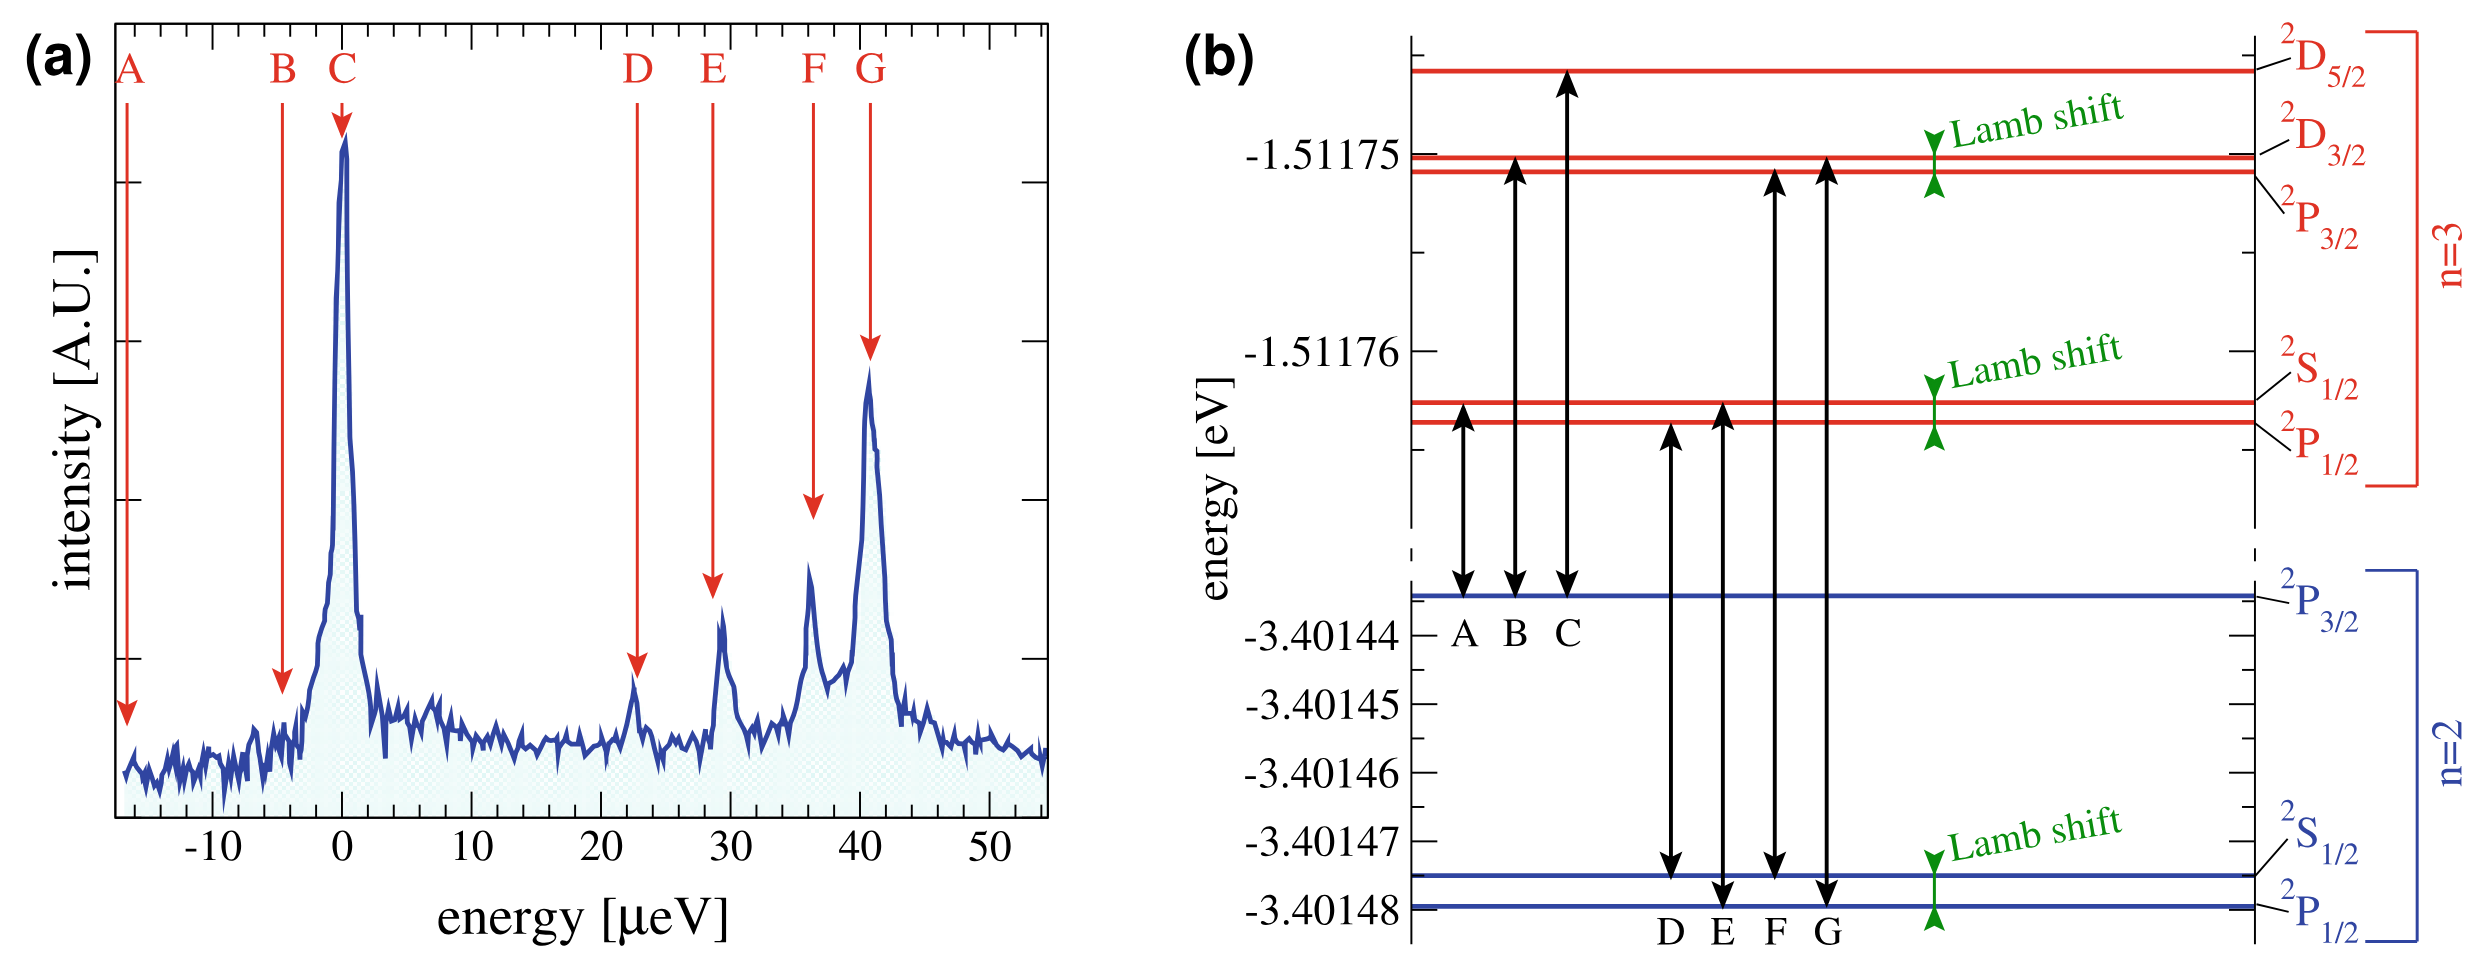
\includegraphics[width = 0.70 \textwidth]{lamb-shift.png}
	\caption{Lamb shift, both theoretical (b) and experimental (a), in the Balmer $ \ch{H}\alpha $ line.}
	\label{img:lamb}
\end{figure}

\section{Struttura iperfine}

Al pari degli elettroni, anche i nuclei hanno un momento angolare di spin $ \ve{I} $, e per molte specie nucleari esso è non-nullo (es.: per il protone $ i = \tfrac{1}{2} $). Per il momento magnetico nucleare sussiste la relazione:
\begin{equation}
	\bs{\mu}_n = g_n \mu_\text{N} \bs{i}
\end{equation}
dove $ \mu_\text{N} \equiv \frac{\hbar q_e}{2m_p} $ è il \textit{magnetone nucleare}. Il valore di $ g_n $ dipende dalla struttura interna del nucleo: ad esempio, per il protone $ g_n \simeq 5.58569 $.\\
Sebbene il campo magnetico nucleare, a parità di distanza, risulti soppresso di $ m_e / m_p \simeq 1 / 1836 $ rispetto a quello elettronico, attraverso questi i momenti magnetici nucleare ed elettronico interagiscono. Dato il fattore $ r^\ell $ in Eq. \ref{eq:1-e-radial}, elettroni con $ \ell > 0 $ hanno probabilità basse di trovarsi vicino al nucleo, dunque l'interazione con essi può essere ignorata; per quanto riguarda gli orbitali $ \ch{S} $, il campo magnetico elettronico è interamente generato dallo spin elettronico $ \ve{S} $ e, analogamente all'interazione spin-orbita, l'interazione tra spin elettronico e spin nucleare è descritta da:
\begin{equation*}
	\mathcal{H}_\text{s-n} = - C \bs{\mu}_n \cdot \bs{\mu}_e = C g_n g_s \mu_\text{N} \mu_\text{B} \bs{i} \cdot \bs{s}
	\qquad \qquad
	C = \frac{2}{3} \frac{1}{4\pi \epsilon_0 c^2} \abs{R_{n,0}(0)}^2 = \frac{2}{3\pi \epsilon_0 c^2} \left( \frac{Z}{an} \right)^3
\end{equation*}
Ricordando che per l'elettrone $ g_s = 2 $, la coupling energy caratteristica risulta essere:
\begin{equation}
	\xi_\text{N} = \frac{4}{3} g_n \frac{Z^3 \alpha^2}{n^3} \frac{m_e}{m_n} E_\text{Ha} \simeq g_n \frac{Z^3}{n^3} \times 1.05\,\mu\text{eV}
\end{equation}
Secondo le regole del momento angolare, $ \ve{I} $ ed $ \ve{S} $ si accoppiano in un \textit{momento angolare atomico} $ \ve{F} = \ve{I} + \ve{S} $, così che per il fattore $ \bs{i} \cdot \bs{s} $ valga, nella coupled basis ($ F^2 $ ed $ F_z $ diagonali), una relazione analoga ad Eq. \ref{eq:sl-coupled-basis}. Ricordando che $ s = \tfrac{1}{2} $, l'interazione tra momenti magnetici nucleare ed elettronico determina uno splitting tra i livelli iperfini $ f = i \pm \tfrac{1}{2} $ pari energeticamente a $ \xi_\text{N} (i \pm \tfrac{1}{2}) $.

\begin{example}{Riga $ 21\,\text{cm} $ dell'idrogeno}{}
	Per $ \ch{^1H} $ si ha $ i = \tfrac{1}{2} $, quindi $ \braket{\bs{i} \cdot \bs{s}} = - \tfrac{3}{4}, \tfrac{1}{4} $ per $ f = 0,1 $ rispettivamente. Nel ground state $ n = 1 $, dunque i due stati iperfini $ f = 0 $ ed $ f = 1 $ risulteranno separati di $ \xi_\text{N} \simeq 5.88\,\mu\text{eV} $: la transizione tra questi livelli sarebbe proibità, poiché $ \Delta \ell = 0 $, ma ha una probabilità non-nulla di avvenire tramite emissione di un fotone con $ \lambda = 2\pi \hbar c \xi_\text{N} \simeq 21\,\text{cm} $ e frequenza $ \nu = \xi_\text{N} (2\pi \hbar)^{-1} \simeq 1.42\,\text{GHz} $. Questa riga spettrale ha valenza storica, in quanto la lunga vita media della transizione (poiché proibita) ne ha permesso la misura della frequenza molto precisa, tant'è che per un periodo è stata usata come standard per l'unità di tempo.
\end{example}

\begin{example}{Struttura iperfine del cesio-137}{}
	Il $ \ch{^{137}Cs} $ è un nuclide con tutte le shell complete ed un elettrone ottico esterno, dunque può essere trattato come un atomo idrogenoide con $ i = \tfrac{7}{2} $ (nuclide dispari-pari). Di conseguenza, per il momento angolare atomico sono possibili solo due valori, dato che $ 3 \le f \le 4 $: la transizioni tra di essi produce un fotone di frequenza $ \nu = 9.192631770 \,\text{GHz} $, e questa riga spettrale e al momento utilizzata come standard per l'unità di tempo.
\end{example}

\section{Transizioni elettroniche}

\subsection{Decadimento spontaneo}

Quando un atomo viene eccitato, esso tenderà a decadere spontaneamente: sperimentalmente, si osserva che non tutte le transizioni procedono allo stesso rate, e ciò può essere spiegato da un'analisi quanto-meccanica dell'interazione del sistema col campo elettromagnetico ambientale. Nell'\textit{approssimazione di dipolo elettrico}\footnotemark, si trova che la probabilità di decadimento radiativo nell'unità di tempo da uno stato iniziale $ \ket{\text{i}} $ ad uno finale $ \ket{\text{f}} $ è:
\begin{equation}
	\gamma_\text{if} = \frac{1}{3\pi \epsilon_0 \hbar^4 c^3} \mathcal{E}_\text{if}^3 \abs{\braket{\text{f} | \ve{d} | \text{i}}}^2
	\label{eq:electron-trans-prob}
\end{equation}
con $ \mathcal{E}_\text{if} \equiv \hbar \omega_\text{if} \defeq E_\text{i} - E_\text{f} $ e $ \ve{d} \equiv - q_e \ve{r} $ l'operatore dipolo elettrico. La dipendenda dall'elemento di matrice $ \braket{\text{f} | \ve{d} | \text{i}} $ impone delle selection rules: le transizioni proibite avvengono con probabilità estremamente inferiori, dato che sono associate a termini di ordine superiore (in $ \alpha $) nell'espansione in multipolo (dipolo magnetico, quadrupolo elettrico, ...).

\footnotetext{Approssimazione valida nel caso in cui la sorgente della radiazione abbia dimensioni molto minori della lunghezza d'onda della radiazione emessa. Essendo $ k = \frac{2\pi}{\lambda} $ e $ \lambda = \frac{hc}{E} $, si ha $ k = \frac{E}{\hbar c} $, dunque tale approssimazione è valida, per $ E \sim 10 - 30 \ev $, se $ k \sim (100 \ang)^{-1} $. Inoltre, si noti che:
\begin{equation}
	\abs{\braket{\text{f} | \ve{p} | \text{i}}}^2 = \abs{\braket{\text{f} | \frac{m}{i\hbar} [\ve{r} , \mathcal{H}] | \text{i}}}^2 = \frac{m^2}{\hbar^2} (E_\text{i} - E_\text{f})^2 \abs{\braket{\text{f} | \ve{r} | \text{i}}}^2 = \frac{m^2}{\hbar^2 q_e^2} \mathcal{E}_\text{if}^2 \abs{\braket{\text{f} | \ve{d} | \text{i}}}^2
	\label{eq:electric-dipole-approx}
\end{equation}}

\begin{theorem}{Electric-dipole selection rule}{}
	Nell'approssimazione di dipolo elettrico per un atomo idrogenoide, le transizioni spontanee ammesse soddisfano:
	\begin{equation}
		\Delta \ell = \pm 1
	\end{equation}

	\tcblower
	
	\begin{proof}
		Esplicitando l'elemento di matrice di $ \ve{d} \equiv -q_e \ve{r} $ in funzione di quello di $ \ve{r} $:
		\begin{equation*}
			\abs{\braket{\text{f} | \ve{r} | \text{i}}}^2 = \abs{\braket{\text{f} | r_x | \text{i}}}^2 + \abs{\braket{\text{f} | r_z | \text{i}}}^2 + \abs{\braket{\text{f} | r_z | \text{i}}}^2
		\end{equation*}
		In funzione delle armoniche sferiche:
		\begin{align*}
			r_x &= r \sin \vartheta \cos \varphi = r \sqrt{\frac{2\pi}{3}} \left[ Y_{1,-1}(\vartheta, \varphi) - Y_{1,1}(\vartheta, \varphi) \right] \\
			r_y &= r \sin \vartheta \sin \varphi = r i \sqrt{\frac{2\pi}{3}} \left[ Y_{1,-1}(\vartheta, \varphi) + Y_{1,1}(\vartheta, \varphi) \right] \\
			r_z &= r \sqrt{\frac{4\pi}{3}} Y_{1,0}(\vartheta, \varphi)
		\end{align*}
		Ne segue che:
		\begin{equation*}
			\abs{\braket{\text{f} | \ve{r} | \text{i}}}^2 = \abs{\braket{\text{f} | r | \text{i}}}^2 \frac{4\pi}{3} \left[ \abs{\braket{\text{f} | Y_{1,-1} | \text{i}}}^2 + \abs{\braket{\text{f} | Y_{1,0} | \text{i}}}^2 + \abs{\braket{\text{f} | Y_{1,1} | \text{i}}}^2 \right]
		\end{equation*}
		Esplicitando in termini della funzione d'onda elettronica:
		\begin{equation*}
			\begin{split}
				\abs{\braket{n_\text{f} , \ell_\text{f} , m_\text{f} | \ve{d} | n_\text{i} , \ell_\text{i} , m_\text{i}}}^2
				& = q_e^2 \abs{\int_0^\infty \dd r\, r^2 R_{n_\text{f} , \ell_\text{f}}(r) R_{n_\text{i} , \ell_\text{i}}(r)}^2 \times \\
				& \times \frac{4\pi}{3} \sum_{m = -1,0,1} \abs{\int_0^\pi \dd \vartheta \, \sin \vartheta \int_0^{2\pi} \dd \varphi \, Y_{\ell_\text{f} , m_\text{f}}^*(\vartheta,\varphi) Y_{1,m}(\vartheta,\varphi) Y_{\ell_\text{i} , m_\text{i}}(\vartheta,\varphi)}^2
			\end{split}
		\end{equation*}
		L'integrale spaziale contribuisce soltanto allo smorzamento delle transizioni con $ \abs{n_\text{i} - n_\text{f}} $ grande, mentre la selection rule è imposta dall'integrale angolare: si noti che esso rappresenza l'overlap angolare tra $ Y_{\ell_\text{f} , m_\text{f}} $ e $ Y_{1,m} Y_{\ell_\text{i} , m_\text{i}} $, ma quest'ultimo può essere scomposto (secondo la decomposizione di Clebsch-Gordan) nella somma di stati con $ \ell = \abs{\ell_\text{i} - 1}, \ell_\text{i}, \ell_\text{i} + 1 $, dunque l'elemento di matrice è non-nullo sono per $ \ell_\text{f} = \ell $. Inoltre, si noti che l'integrale si annulla per $ \ell_\text{f} = \ell_\text{i} $: in tal caso, la parità dell'integranda sarebbe $ (-1)^{\ell_\text{i}} (-1)^1 (-1)^{\ell_\text{i}} = -1 $, dunque il suo integrale su tutto l'angolo solido è nullo. Gli unici valori possibili sono dunque $ \ell_\text{f} = \ell_\text{i} \pm 1 $, ovvero la selection rule cercata.
	\end{proof}
\end{theorem}

Essendo l'operatore dipolo elettrico associato a $ \ell = 1 $, si ha che $ m = -1,0,1 $; di conseguenza, si ottiene una selection rule anche sulla proiezione del momento angolare orbitale:
\begin{equation}
	\Delta m = 0, \pm 1
	\label{eq:1-e-el-dip-tr-m}
\end{equation}
Inoltre, dato che $ \ve{d} $ agisce come l'identità sullo spazio degli spin, si hanno:
\begin{equation}
	\Delta s = 0
	\qquad \qquad
	\Delta m_s = 0
	\label{eq:1-e-el-dip-tr-spin}
\end{equation}
È anche possibile esprimere la selection rule sulla base accoppiata, ottenendo:
\begin{equation}
	\Delta j = 0 , \pm 1
	\qquad \qquad
	\Delta m_j = 0 , \pm 1
\end{equation}
Una volta determinate le transizioni possibili, si può dare una stima del decay rate dall'Eq. \ref{eq:electron-trans-prob}, usando $ \mathcal{E}_\text{if} \simeq Z^2 E_\text{Ha} $ e $ \abs{\braket{\text{f} | \ve{d} | \text{i}}} = q_e a_0 / Z $:
\begin{equation}
	\gamma_\text{if} = \frac{\mathcal{E}_\text{if}^3 \abs{\braket{\text{f} | \ve{d} | \text{i}}}^2}{3\pi \epsilon_0 \hbar^4 c^3} \simeq \frac{Z^4 E_\text{Ha}^2}{\epsilon_0 \hbar^4 c^3} \hbar \omega_\text{if} \frac{q_e^2 a_0^2}{Z^2} \simeq \frac{e^2 Z^2}{(\hbar c)^3} e^4 \omega_\text{if} = Z^2 \alpha^3 \omega_\text{if}
	\label{eq:electric-dipole-decay-rate}
\end{equation}
dato che $ E_\text{Ha} a_0 = e^2 $ e $ \alpha = e^2 / (\hbar c) $. Per un atomo idrogenoide $ \omega_\text{if} \simeq Z^2 \cdot 10^{16} \,\text{Hz} $, dunque si trova un tempo di decadimento dell'ordine $ \gamma_\text{if}^{-1} \simeq Z^{-4} \,\text{ns} $.

\begin{example}{Doppietto giallo del sodio}{}
	L'atomo di sodio presenta 11 elettroni: 10 interni in shell complete ed 1 esterno in 3s. Come in tutti gli altri atomi alcalini, l'elettrone esterno si trova più lontano dal nucleo rispetto alle shell interne ed è chiamato \textit{elettrone ottico}, poiché tipicamente le sue transizioni cadono nel visibile. Il potenziale a cui è soggetto l'elettrone ottico può essere visto come Coulombiano con un $ Z_\text{eff} $ efficacie: a grandi distanze dal nucleo $ Z_\text{eff} \simeq Z - (Z-1) = 1 $, mentre avvicinandosi ad esso $ Z_\text{eff} = Z_\text{eff}(r) $, il che rompe la degenerazione accidentale (l'energia è $ E = E(n,\ell) $). \\
	Nel caso del sodio, il tipico doppietto giallo del suo spettro d'emissione è dovuto alla transizione ottica ($ \Delta \ell = \pm 1 $) più piccola possibile per l'elettrone ottico, ovvero $ \text{3p} \rightarrow \text{3s} $ ($ \Delta E \sim 2\ev $). In particolare, sono presenti due righe a causa dell'interazione spin-orbita ($ \Delta E \sim 2.1 \,\text{meV} $), poiché le transizioni possibili sono due: $ \ch{^3P}_{3/2} \rightarrow \ch{^3S}_{1/2} $ ($ \lambda = 589.0 \,\text{nm} $) e $ \ch{^3P}_{1/2} \rightarrow \ch{^3S}_{1/2} $ ($ \lambda = 589.6 \,\text{nm} $).
\end{example}

\subsection{Decadimento stimolato}

In generale, un sistema immerso in un campo elettromagnetico descritto dai potenziali $ \phi $ ed $ \ve{A} $ è descritto dall'Hamiltoniana:
\begin{equation}
	\mathcal{H} = \frac{1}{2m} \left( \ve{p} - \frac{q}{c} \ve{A} \right)^2 + q \phi
\end{equation}
Nel caso dell'atomo idrogenoide:
\begin{equation}
	\mathcal{H} = \frac{1}{2m_e} \left( \ve{p} + \frac{e}{c} \ve{A} \right)^2 + \frac{1}{2M} \left( \ve{P} - \frac{Ze}{c} \ve{A} \right)^2 - \frac{Ze}{\abs{\ve{r} - \ve{R}}}
\end{equation}
Trascurando $ \frac{1}{M} \ll \frac{1}{m_e} $, ponendo $ \ve{R} = \ve{0} $ e scegliendo un gauge $ [\nabla , \ve{A}] = 0 $:
\begin{equation*}
	\begin{split}
		\mathcal{H}
		& \simeq \frac{1}{2m_e} \left( \ve{p} + \frac{e}{c} \ve{A} \right)^2 - \frac{Ze}{r} = \frac{1}{2m_e} \left[ -\hbar^2 \lap - i \frac{\hbar e}{c} (\nabla \cdot \ve{A} + \ve{A} \cdot \nabla) + \frac{e^2}{c^2} \ve{A}^2 \right] - \frac{Ze}{r} \\
		& = \frac{\hbar^2}{2m_e} \left[ -\lap - 2i \frac{\alpha}{e} \ve{A} \cdot \nabla + \frac{\alpha^2}{e^2} \ve{A}^2 \right] - \frac{Ze}{r} = \underbrace{- \frac{\hbar^2}{2m_e} \lap - \frac{Ze}{r}}_{\mathcal{H}_0} \underbrace{- i \frac{\hbar^2}{m_e} \frac{\alpha}{e} \ve{A} \cdot \nabla}_{V} + \underbrace{\frac{\hbar^2}{2m_e} \frac{\alpha^2}{e^2} \ve{A}^2}_{\sim \, \alpha^2}
	\end{split}
\end{equation*}
L'ultimo termine può essere trascurato, dunque il problema può essere trattato perturbativamente al prim'ordine (nell'approssimazione di campo debole). Per semplificare la trattazione, si adottano le unità atomiche $ \hbar = m_e = e = 1 , c = \alpha^{-1} \simeq 137 $:
\begin{equation}
	\mathcal{H} \simeq - \frac{1}{2} \lap - \frac{Z}{r} - i \alpha \ve{A} \cdot \nabla
\end{equation}
La dipendenza temporale degli autostati di $ \mathcal{H} $ non è più banale, in quanto la perturbazione determina una dipendenza temporale:
\begin{equation}
	\psi(t,r) = \sum_{n \in \N} c_n(t) e^{-i E_n t} \psi_n(r)
	\label{eq:1-e-pert-autof}
\end{equation}
dove $ \psi_n(r) $ sono gli stati stazionari di $ \mathcal{H}_0 $ e al prim'ordine:
\begin{equation}
	c_n(t) \simeq c_n^{(0)} + c_n^{(1)}(t)
	\label{eq:1-e-pert-coeff}
\end{equation}

\begin{proposition}{Coefficienti perturbativi}{}
	Per un potenziale del tipo:
	\begin{equation}
		\ve{A}(t,\ve{r}) = \ve{A}_0 e^{i (\ve{k}_0 \cdot \ve{r} - \omega_0 t + \varphi_0)} + \text{c.c.} = 2 \ve{A}_0 \cos (\ve{k}_0 \cdot \ve{r} - \omega_0 t + \varphi_0)
	\end{equation}
	i coefficienti nello sviluppo perturbativo per una transizione tra due stati stazionari $ \ket{n} , \ket{m} $ sono:
	\begin{equation}
		\begin{split}
			c_n^{(1)}(t) = - \alpha t \ve{A}_0 \cdot \bigg[
			& \ve{M}_{nm}(\ve{k}_0) \exp \left( i \frac{\omega_{nm} - \omega_0}{2} t + i \varphi_0 \right) \sinc \left( \frac{\omega_{nm} - \omega_0}{2} t \right) + \\
			& \qquad - \ve{M}_{mn}^*(\ve{k}_0) \exp \left( i \frac{\omega_{nm} + \omega_0}{2} t + i \varphi_0 \right) \sinc \left( \frac{\omega_{nm} + \omega_0}{2} t \right) \bigg]
			\label{eq:1-e-big-coeff}
		\end{split}
	\end{equation}
	con $ \ve{M}_{nm}(\ve{k}_0) \equiv \braket{n | e^{i \ve{k}_0 \cdot \ve{r}} \nabla | m} $.

	\tcblower

	\begin{proof}
		L'equazione di Schrödinger per l'autofunzione \ref{eq:1-e-pert-autof} diventa:
		\begin{equation*}
			\sum_{m \in \N} c_m(t) e^{-i E_m t} \mathcal{H} \psi_m(r) = i \sum_{m \in \N} \left[ \frac{dc_m(t)}{dt} - i E_m c_m(t) \right] e^{-i E_m t} \psi_m(r)
		\end{equation*}
		Moltiplicando a sinistra per $ \psi_n^*(r) $ ed integrando su tutto lo spazio:
		\begin{equation*}
			\sum_{m \in \N} c_m(t) e^{-i E_m t} \left( \delta_{nm} + \braket{n | V | m} \right) = \sum_{m \in \N} \left[ i \frac{dc_m(t)}{dt} + E_m c_m(t) \right] e^{-i E_m t} \delta_{nm}
		\end{equation*}
		Semplificando, si trova:
		\begin{equation*}
			\frac{dc_n(t)}{dt} = -i \sum_{m \in \N} c_m(t) e^{i \mathcal{E}_{nm} t} \braket{n | V | m}
		\end{equation*}
		Dall'Eq. \ref{eq:1-e-pert-coeff}, dato che $ c_n^{(1)} \ll c_n^{(0)} $:
		\begin{equation*}
			\frac{dc_n^{(1)}(t)}{dt} = -i \sum_{k \in \N} c_k^{(0)}(t) e^{i \mathcal{E}_{nk} t} \braket{n | V | k}
		\end{equation*}
		Per uno stato iniziale stazionario $ \ket{m} $ si ha $ c_k^{(0)} = \delta_{km} $, dunque:
		\begin{equation*}
			\frac{dc_n^{(1)}(t)}{dt} = -i e^{i \mathcal{E}_{nm} t} \braket{n | V | m} = - e^{i \mathcal{E}_{nm} t} \alpha \ve{A}_0 \cdot \left[ \braket{n | e^{i\ve{k}_0 \cdot \ve{r}} \nabla | m} e^{-i \omega_0 t + \varphi_0} + \text{c.c.} \right]
		\end{equation*}
		Essendo $ \nabla $ anti-hermitiano, $ \ve{M}_{nm}^*(\ve{k}_0) = - \ve{M}_{mn}(\ve{k}_0) $, ovvero:
		\begin{equation*}
			\frac{dc_n^{(1)}(t)}{dt} = - \alpha \ve{A}_0 \cdot \left[ \ve{M}_{nm}(\ve{k}_0) e^{i (\omega_{nm} - \omega_0) t + i \varphi_0} - \ve{M}_{mn}^*(\ve{k}_0) e^{i (\omega_{nm} + \omega_0) t - i \varphi_0} \right]
		\end{equation*}
		Integrando:
		\begin{equation*}
			\int_0^t dt' e^{i \beta t'} = \frac{e^{i\beta t} - 1}{i \beta} = \frac{i (1 - \cos \beta t) + \sin \beta t}{\beta} = \frac{2}{\beta} e^{i \beta \frac{t}{2}} \sin \left( \beta \tfrac{t}{2} \right) = \frac{t e^{i\beta \frac{t}{2}} \sin \left( \beta \frac{t}{2} \right)}{\beta \frac{t}{2}}
		\end{equation*}
		Utilizzando questo risultato per risolvere l'ODE per $ c_n^{(1)}(t) $ si ottiene la tesi.
	\end{proof}
\end{proposition}

Si ottiene quindi che, per un sistema inizialmente in uno stato stazionario $ \ket{m} $:
\begin{equation}
	\psi(t,r) = \psi_m(r) + \sum_{n \in \N} c_{nm}(t) e^{- i E_n t} \psi_n(r)
\end{equation}
con $ c_{nm}(t) \equiv c_n^{(1)}(t) $ come in Eq. \ref{eq:1-e-big-coeff}. La probabilità di transizione da $ \ket{m} $ a $ \ket{n} $, con $ n \neq m $, sarà dunque $ P_{nm}(t) = \abs{c_{nm}(t)}^2 $.

\paragraph{Risonanza}

Essendo $ \omega_0 $ la pulsazione della radiazione incidente, in base al valore di $ \omega_{nm} $ (differenza tra i due livelli energetici) si hanno due possibili risonanze (a seconda di quale termine domina in Eq. \ref{eq:1-e-big-coeff}):
\begin{itemize}
	\item $ \omega_{nm} \approx \omega_0 $: domina il primo termine, ovvero si ha risonanza per il processo di assorbimento (eccitamento) con transizione da $ \omega_m $ a $ \omega_n = \omega_m + \omega_0 $;
	\item $ \omega_{nm} \approx - \omega_0 $: domina il secondo termine, ovvero si ha risonanza per il processo di emissione (decadimento) con transizione da $ \omega_m $ a $ \omega_n = \omega_m - \omega_0 $.
\end{itemize}
Inoltre, si noti che $ \sinc{x} \rightarrow 0 $ per $ x \rightarrow \infty $, dunque col passare del tempo le probabilità di transizione per $ n \neq m $ tendono ad annullarsi; ciò è legato alla natura della radiazione emessa: inizialmente essa è non-monocromatica, ma col passare del tempo tende a diventare sempre più monocromatica.

\paragraph{Golden rule di Fermi}

È possibile definire la probabilità di transizione per unità di tempo sia nel caso dell'assorbimento che in quello dell'emissione:
\begin{align*}
	P_\text{a}(t) &= \abs{c_{nm}(t)}^2 \simeq \alpha^2 t^2 A_0^2 \abs{\bs{\epsilon} \cdot \ve{M}_{nm}(\ve{k}_0)}^2 \sinc^2 \left( \tfrac{\omega_{nm} - \omega_0}{2} t \right) \sim 2\pi \alpha^2 t A_0^2 \abs{\bs{\epsilon} \cdot \ve{M}_{nm}(\ve{k}_0)}^2 \delta(\tfrac{\omega_{nm} - \omega_0}{2}) \\
	P_\text{e}(t) &= \abs{c_{nm}(t)}^2 \simeq \alpha^2 t^2 A_0^2 \abs{\bs{\epsilon} \cdot \ve{M}_{mn}^*(\ve{k}_0)}^2 \sinc^2 \left( \tfrac{\omega_{nm} + \omega_0}{2} t \right) \sim 2\pi \alpha^2 t A_0^2 \abs{\bs{\epsilon} \cdot \ve{M}_{mn}^*(\ve{k}_0)}^2 \delta(\tfrac{\omega_{nm} + \omega_0}{2})
\end{align*}
dove $ \bs{\epsilon} = \ve{A}_0 / A_0 $ è la polarizzazione della radiazione incidente e $ \delta(x) = \frac{1}{2\pi} \lim_{t \rightarrow \infty} t \sinc^2(xt) $. Definendo l'intensità della radiazione incidente come $ I_0 \equiv A_0^2 \omega_0^2 / (2\pi c) $, si ottiene la golden rule di Fermi:
\begin{align*}
	P_\text{a}(t) &\simeq 4\pi \alpha^2 t \abs{\bs{\epsilon} \cdot \ve{M}_{nm}(\ve{k}_0)}^2 \frac{I_0}{\omega_0^2} \delta(\omega_{nm} - \omega_0) \\
	P_\text{e}(t) &\simeq 4\pi \alpha^2 t \abs{\bs{\epsilon} \cdot \ve{M}_{mn}^*(\ve{k}_0)}^2 \frac{I_0}{\omega_0^2} \delta(\omega_{nm} + \omega_0)
\end{align*}
Si noti che l'unico termine distinto è la $ \delta $ di conservazione dell'energia, la quale può essere scritta in maniera unificata come $ \delta(\omega_\text{f} - \omega_\text{i}) $. Inoltre, si vede che la probabilità di transizione diverge alla risonanza: questo però non è un problema, in quanto non esistono sorgenti puramente monocromatiche, in quanto dovrebbero emettere per un tempo infinito; più realisitcamente, si ha una distribuzione d'intensità attorno a $ \omega_0 $, così da scrivere:
\begin{equation*}
	\frac{I_0}{\omega_0^2} \delta(\omega_{nm} \pm \omega_0) \longrightarrow \int_{-\infty}^{+\infty} d\omega\, \frac{I(\omega)}{\omega^2} \delta(\omega_{nm} \pm \omega_0) = \frac{I(\omega_{nm})}{\omega_{nm}^2}
\end{equation*}
Utilizzando l'approssimazione di dipolo elettrico Eq. \ref{eq:electric-dipole-approx}, si trova che il rate di transizione $ \gamma_\text{if} \equiv P_\text{if} / t $ può essere scritto come:
\begin{equation*}
	\gamma_\text{if} = 4\pi \alpha^2 \abs{\braket{\text{f} | e^{i \ve{k}_0 \cdot \ve{r}} \nabla | \text{i}}}^2 \frac{I(\omega_\text{if})}{\omega_\text{if}^2} \simeq 4\pi \alpha^2 \abs{\braket{\text{f} | \ve{p} | \text{i}}}^2 \frac{I(\omega_\text{if})}{\omega_\text{if}^2} = 4\pi \alpha^2 \omega_\text{if}^2 \abs{\braket{\text{f} | \ve{d} | \text{i}}}^2 \frac{I(\omega_\text{if})}{\omega_\text{if}^2}
\end{equation*}
Si trova dunque:
\begin{equation}
	\gamma_\text{if} = 4\pi \alpha^2 I(\omega_\text{if}) \abs{\braket{\text{f} | \ve{d} | \text{i}}}^2
\end{equation}
A differenza dell'emissione spontanea, che è $ \sim \mathcal{E}_\text{if}^3 $, quella stimolata è $ \sim \mathcal{E}_\text{if}^2 $, dunque l'emissione spontanea diventa più probabile di quella stimolata all'aumentare della differenza energetica.

\section{Campo magnetico esterno}

Maggiori informazioni su una specie atomica possono essere ricavate immergendo il campione in un campo magnetico uniforme e studiandone lo spettro. Il momento magnetico atomico totale può essere scritto come:
\begin{equation}
	\bs{\mu} = \bs{\mu}_\ell + \bs{\mu}_s = - \mu_\text{B} ( g_\ell \bs{\ell} + g_s \bs{s}) \simeq - \mu_\text{B} (\bs{\ell} + 2 \bs{s})
\end{equation}
L'Hamiltoniana di coupling con un campo magnetico esterno, WLOG $ \ve{B} = B \hat{\ve{e}}_z $, è:
\begin{equation}
	\mathcal{H}_\text{magn} = - \bs{\mu} \cdot \ve{B} = \mu_\text{B} B (\ell_z + 2s_z)
\end{equation}
Si vede che $ \mathcal{H}_\text{magn} $ è diagonalizzabile nella uncoupled basis $ \ket{\ell, m, s, m_s} $, mentre $ \mathcal{H}_\text{s-o} $ lo è nella coupled basis $ \ket{\ell, s, j, m_j} $: dato che $ [\mathcal{H}_\text{magn} , \mathcal{H}_\text{s-o}] \neq 0 $, essi non sono simultaneamente diagonalizzabili, ma vanno diagonalizzati di volta in volta in ogni sottospazio $ (2\ell + 1)(2s + 1) $-dimensionale a $ n,\ell,s $ fissati.
È però possibile studiare i casi limite per le energie caratteristiche $ \mu_\text{B} B $ e $ \xi $.

\subsection{Limite Paschen-Back}

Nel limite $ \mu_\text{B} B \gg \xi $ in cui domina il campo magnetico esterno, la diagonalizzazione è diretta poiché si usa la uncoupled basis:
\begin{equation}
	\Delta E_\text{magn}(m,m_s) = \braket{m,m_s | \mathcal{H}_\text{magn} | m,m_s} = \mu_\text{B} B (m + 2m_s)
\end{equation}
mentre la correzione dovuta a $ \mathcal{H}_\text{s-o} $ può essere trattata perturbativamente. \\
Il valore di $ B $ per cui si può effettuare questa approssimazione dipende dall'atomo considerato e dal livello energetico: ad esempio, considerando la shell $ \text{2p} $, per $ \ch{H} $ si ha $ B \gg 0.5 \,\text{T} $, mentre per $ \ch{He}^+ $ si ha $ B \gg 8 \,\text{T} $, a causa della dipendenza da $ Z^4 $ in Eq. \ref{eq:1-e-int-spin-orb}.

\subsection{Limite Zeeman}

Il limite $ \mu_\text{B} B \ll \xi $ in cui domina l'interazione spin-orbita è quello più comune e in esso la simmetria sferica subisce solo una debole perturbazione. Gli stati $ \ket{\ell,s,j,m_j} $ nella coupled basis sono dunque autostati approssimati di $ \mathcal{H}_\text{s-o} + \mathcal{H}_\text{magn} $, mentre la correzione al prim'ordine dell'energia è:
\begin{equation}
	\Delta E_\text{magn}(j,m_j) \simeq \braket{j,m_j | \mathcal{H}_\text{magn} | j,m_j} = g_j \mu_\text{B} B m_j
\end{equation}
dove $ g_j $ è il fattore di Landé (Eq. \ref{eq:lande-g-factor}).

\subsection{Linee spettrali}

Sperimentalmente, si confermano le considerazioni teoriche sia esatte che approssimate. Prendendo ad esempio un campione di $ \ch{H} $, applicando un campo magnetico sufficientemente potente si osserva una triplicazione delle linee spettrali ($ \Delta m = 0, \pm 1 $), in accordo con l'effetto Paschen-Back, mentre applicando un campo magnetico debole si osserva l'effetto Zeeman (Fig. \ref{zeeman-effect}).

\begin{figure}
	\centering
	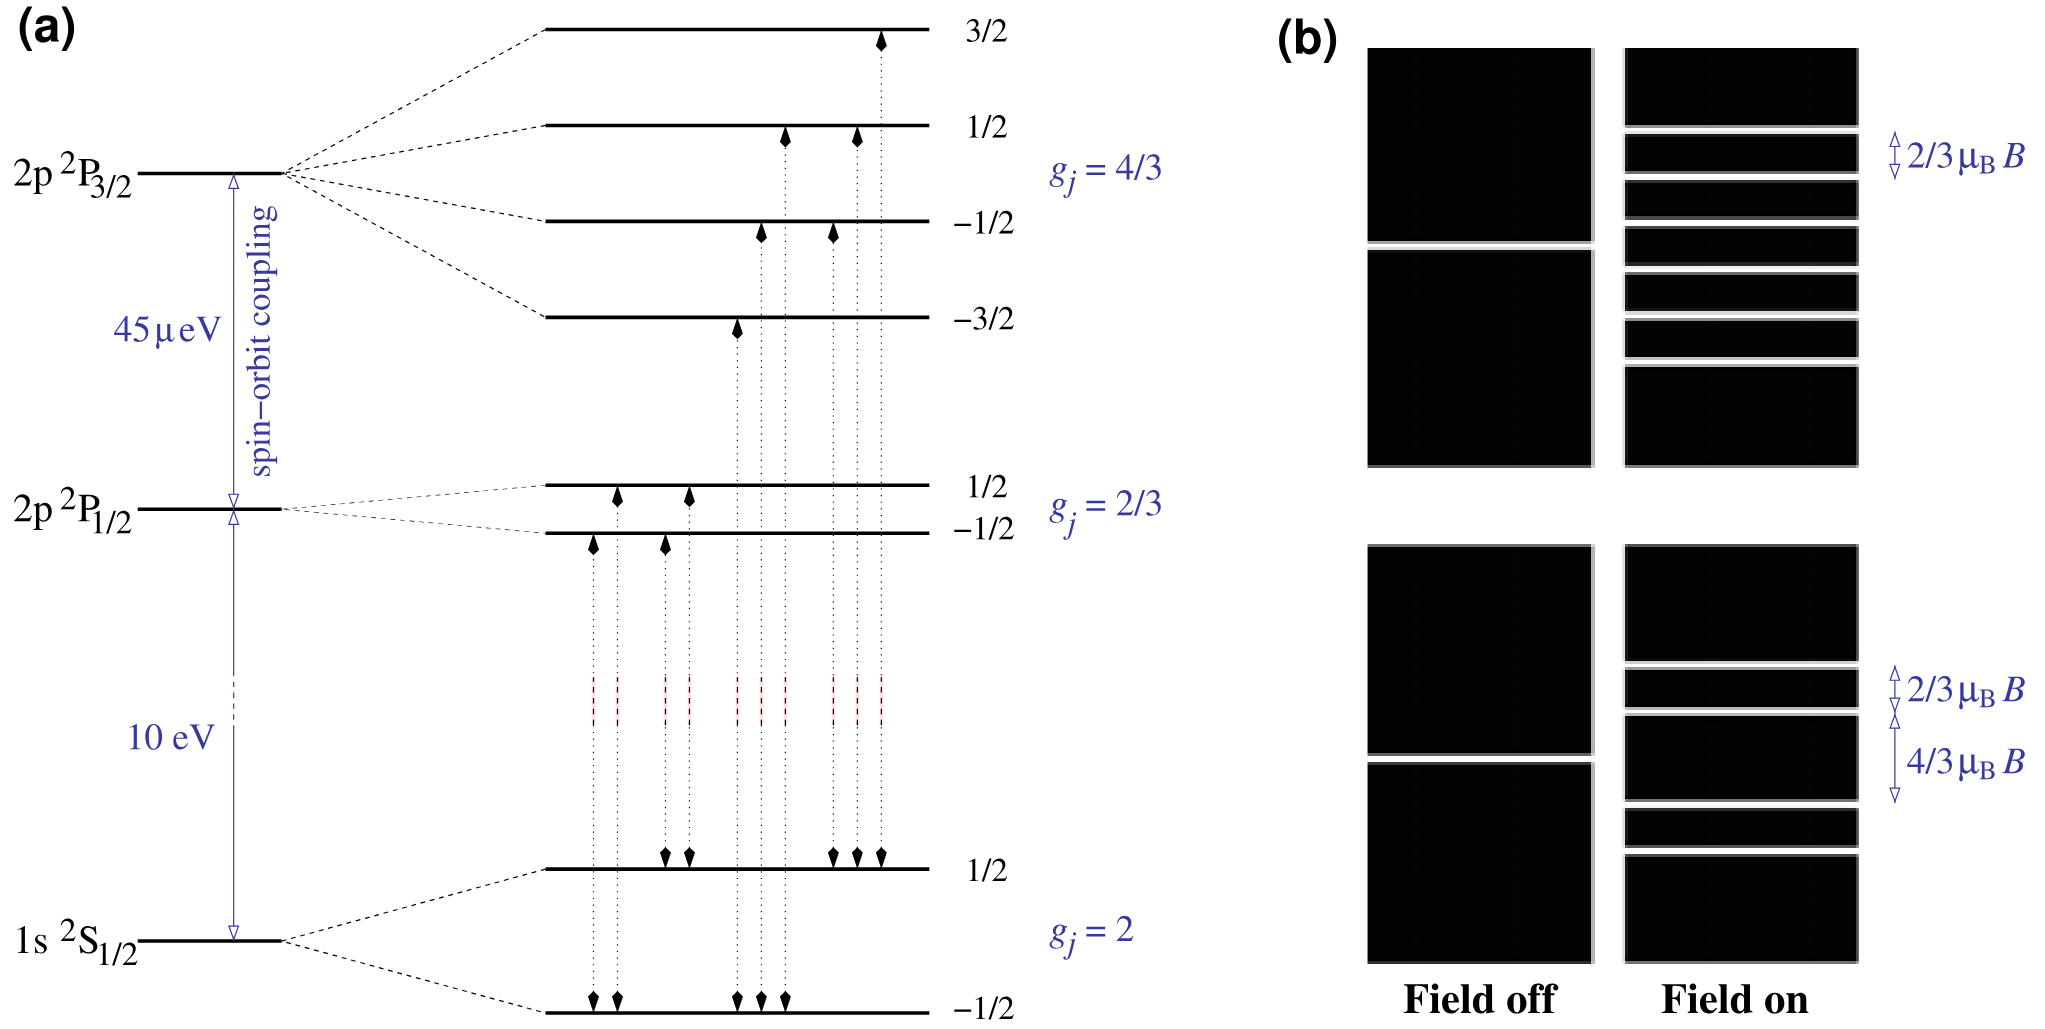
\includegraphics[width = 0.85 \textwidth]{zeeman-effect.png}
	\caption{Zeeman split of the lowest Lyman line of $ \ch{H} $.}
	\label{zeeman-effect}
\end{figure}

Nel regime intermedio $ \mu_\text{B} B \sim \xi $, nessuna delle due basi riesce a dare una descrizione accurata dei livelli energetici. Ad esempio, Fig. \ref{mag-field-int} mostra lo splitting pattern dei 6 stati $ \ch{^2P} $ in funzione dell'intensità del campo magnetico.

\begin{figure}[!b]
	\centering
	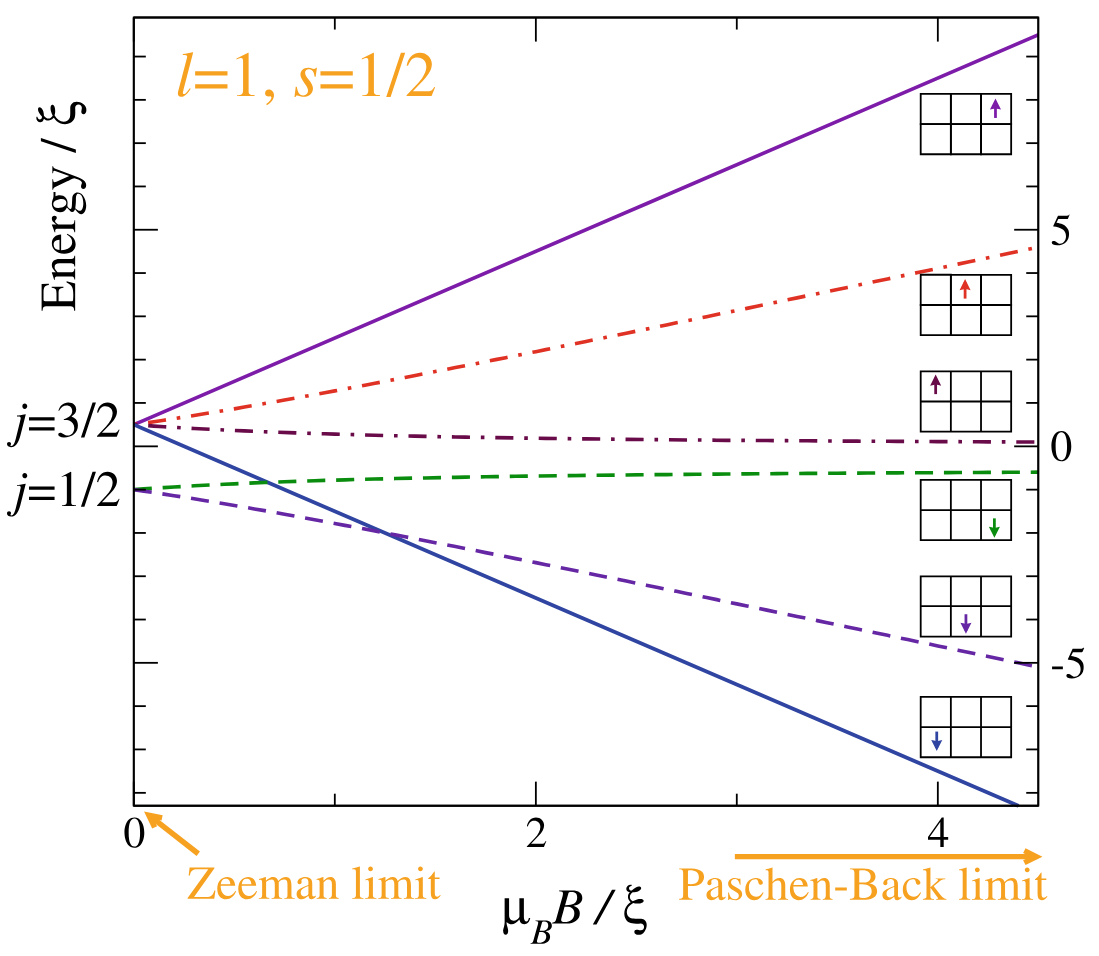
\includegraphics[width = 0.50 \textwidth]{mag-field-int.png}
	\caption{Combined spin-orbit and magnetic splittings of $ \ch{^2P} $.}
	\label{mag-field-int}
\end{figure}










